\chapter{Configurations of lines}\label{configs}
\section{Surfaces including m-crosses}

\begin{figure}
    \centering
    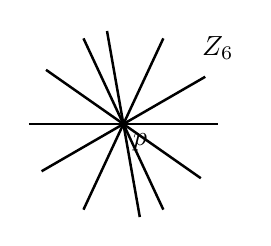
\begin{tikzpicture}[scale=0.4]
% Six lines passing through a common point p at the origin
% Draw the six lines without inline labels
\foreach \theta in {115,-80,65,-35,30,0} {
    \draw[rotate=\theta, line width=0.9pt] (-3,0) -- (3,0);
}
% Common intersection point p
\fill (0,0) circle (2pt) node[below right] {$p$};

% Optional label
\node at (3,2.4) {$Z_6$};
\end{tikzpicture}
  \caption{An example of a 6-cross in $\mathbb{P}^3$.}
  \label{fig:Z_6}
\end{figure}

In this section we will study the problem of finding a smooth hypersurface $X_d \subset \mathbb{P}^3$ of degree $d$, containing an \emph{$m$-cross}. 

\begin{definition}
    An $m$-cross is a union of $m$ distinct lines $l_1, l_2, \dots, l_m$ in $\mathbb{P}^3$ which intersect at a common point $p$ and lying in a common plane $H$. We will write $Z_m = \bigcup_{i=1}^m l_i$.
\end{definition}

We require the lines to lie in a plane because if this is not true, then the point $p$ gives rise to a tangent space of dimension 3, which cannot be included in a surface in $\mathbb{P}^3$. 

\todo[inline]{Gjør dette argumentet rigorøst. Se notat fra 6.11.}

It is worth noting the specific question we are asking, which is that given an $m$-cross, does there exist a smooth hypersurface of degree $d$ including it. We do not ask whether an $m$-cross is to be expected inside a general hypersurface.

\begin{remark}\label{rem:autPm}
    Note that for automorphisms of $\mathbb{P}^3$, lines are sent to lines. Therefore, we can study the lines $l_1 = (\alpha : \beta : 0 : 0), \ l_2 = (\alpha : 0 : \gamma : 0), \ l_3=(\alpha: \delta : \lambda_3 \delta: 0), \dots, l_m = (\alpha : \delta : \lambda_m \delta : 0)$ for $\lambda_i \in \mathbb{N}$, where $\alpha$, $\beta$, $\gamma$, and $\lambda_i$ are parameters which vary, by taking the automorphism of $\mathbb{P}^3$ which sends these lines to the given lines, and then study the hypersurface of degree $d$ in $\mathbb{P}^3$ which contains these lines. This automorphism will also take a smooth hypersurface of degree $d$ to a smooth hypersurface of degree $d$, so showing properties for lines in this form is sufficient for the general case. In this way, we can assume without loss of generality that the plane $H$ containing the lines is given as $H = V(x_3)$, and we notice that a line $l_i = V(H)\cap V(g_i)$ for some $g_i \in \mathbb{C}[x_0,x_1,x_2,x_3]$. The lines given above can then be described as the zero loci of the following polynomials: 
    \begin{equation}\label{eq:li}
        l_1 = V(x_3, x_2), \ l_2 = V(x_3, x_1), \ l_3 = V(x_3, x_1 - \lambda_3 x_2), \ \dots, \ l_m = V(x_3, x_1 - \lambda_m x_2).
    \end{equation}
\end{remark}

We are interested in both the existence and non-existence of degree $d$ hypersurfaces containing $m$-crosses. We first consider surfaces with degree less than $k$, but more than 1 (degree 1 provides us a simple choice of surface including an $m$-cross, namely $H$).

\begin{lemma}\label{lem:H}
    If $S$ is a smooth surface in $\mathbb{P}^3$ of degree $d > 1$, it does not contain a plane.
\end{lemma}
\begin{proof}
    Assume for contradiction that $S = V(g)$ contains a plane $H$. We let $H = V(x_3)$ without loss of generality, by \cref{rem:autPm}. Then $x_3$ divides $g$, and we write $g = x_3 h$ for some $h \in \mathbb{C}[x_0,x_1,x_2,x_3]_{d-1}$. We then use the Jacobi criterion \cite[Proposition 16.16]{EO25} on $x_3 h$, and get that $S$ is singular on the whole of $V(x_3) \cap V(h)$. This is non-empty by Bezout's theorem (\cref{thm:bezout}), giving a contradiction. (Use $d>1$ to see that $\text{deg}(h) = d-1 > 0$)(!?). 
\end{proof}
\todo[inline]{Dobbeltsjekk hvis tid.}

\begin{lemma}
    Given an $m$-cross, there does not exist any smooth hypersurface of degree $1 < d < m$ such that the lines are contained in the hypersurface.
\end{lemma}
\begin{proof}
    Assume for contradiction that there exists a smooth hypersurface of degree $1 < d < m$ such that the lines are contained in the hypersurface. Then we can fix another line $\ell$ in $H$, which does not intersect $p$, and which does not lie in the hypersurface $X_d$ by \cref{lem:H}. $\ell$ will intersect each of the lines at a point $p_i$, all being distinct since the lines only intersect in $p$. $\ell$ will also intersect $X_d$ at the points $p_i$, thus intersecting the hypersurface at $m$ points. By Bezout's theorem (\cref{thm:bezout}), the intersection of a line with a hypersurface of degree $d$ is at most $d$ points, giving a contradiction. 
\end{proof}

We now move on to the case of existence, with the following proposition:

\begin{proposition}
    For a given $m$-cross, we can find a smooth hypersurface of degree $m$ such that the lines are contained in the hypersurface.
\end{proposition}
\begin{proof}
    Let $\mathfrak{L}$ be the linear system of hypersurfaces of degree $m$ in $\mathbb{P}^3$ containing the lines $l_1, \dots, l_m$. Recall that Bertini's theorem, \cref{thm:bertini}, tells us that the general member of $\mathfrak{L}$ is smooth outside the base locus of $\mathfrak{L}$. We can therefore narrow our search of singularities to the base locus. The base locus of $\mathfrak{L}$ is the union of the lines $l_1, \dots, l_m$. To see why, consider a point $x \in \mathbb{P}^3$ which does not lie on one of the lines. We want to show that for each of these points, we can find a surface which excludes the points, but includes the surface. First, if the point is not in the plane $H$, we can exclude it by the plane itself, so we assume the point lies in $H$, but not in one of the lines. 
    Then we consider the loci which define the lines, as discussed in \cref{rem:autPm}, denoted $l_i = V(H) \cap V(g_i)$. Then all the lines $l_1, \dots l_m$ are included in $V(\Pi_{i=1}^m g_i)$, while $x$ is not. 
    % Then we consider the equations of the lines from \ref{eq:li}, denoted $l_i = V(g_i)$ for $g_i \in \mathcal{C}[x_0,x_1,x_2]$. Then all the lines $l_1, \dots l_m$ are included in $V(\Pi_{i=1}^m g_i)$, while $x$ is not. 
    
    Since we know exactly the base locus, we want to find a function $f \in \mathbb{C}[x_0, x_1, x_2, x_3]_m$ such that $V(f)$ is smooth on the lines $l_1, \dots, l_m$. Bertini's theorem then gives us that we can find a hypersurface which is also smooth outside the base locus of $\mathfrak{L}$.

   Now we take inspiration from \ref{eq:li}, and study the function $f = g(x_1, x_2) + h(x_0, x_3)$, where $h = x_0^{m-1}x_3$ and $g = \prod l_i = x_1x_2 \prod_{i=3}^k (x_1 - \lambda_i x_2)$, giving the following polynomial:
    \[
        f(x_0, x_1, x_2, x_3) = x_1x_2 \prod_{i=3}^m (x_1 - \lambda_i x_2) + x_0^{m-1}x_3.
    \]
    We can see that $f$ is a polynomial of degree $m$, and that $V(f)$ includes the lines $l_1, \dots, l_m$, since $f(\alpha: \beta: 0: 0) = f(\alpha: 0: \gamma: 0) = f(\alpha: \delta: \lambda_i \delta: 0) = 0$. We must then check that $f$ is smooth on the base locus of $\mathfrak{L}$, which is to check that $\bigcap_{i=0}^3 (\partial_i f = 0) = \emptyset$. 
    
    The derivatives are given as follows:
    \begin{align*}
        \partial_0 f &= \partial_0 g + \partial_0 h = 0 + (m-1)x_0^{m-2}x_3 = (m-1)x_0^{m-2}x_3, \\
        \partial_1 f &= \partial_1 g + \partial_1 h = x_2 \prod_{i=3}^m (x_1 - \lambda_i x_2) + x_1x_2 \sum_{i=3}^m \prod_{\substack{j=3 \\ j \neq i}}^m (x_1 - \lambda_j x_2), \\
        \partial_2 f &= \partial_2 g + \partial_2 h = x_1 \prod_{i=3}^m (x_1 - \lambda_i x_2) +  x_1x_2 \sum_{i=3}^m (-\lambda_i) \cdot \prod_{\substack{j=3 \\ j \neq i}}^m (x_1 - \lambda_j x_2), \\
        \partial_3 f &= \partial_3 g + \partial_3 h = 0 + x_0^{m-1} = x_0^{m-1}.
    \end{align*}

    We then find that on the base locus of $\mathfrak{L}$, the following hold:
    \begin{itemize}
        \item $\partial_0 f = 0$ on the entire base locus, since it contains the factor $x_3$, which is 0 on the entire plane.
        \item $\partial_1 f = 0$ on the line $l_0 = (\alpha : \beta : 0 : 0)$, since $\partial_1 f$ contains the factor $x_2$, and is non-zero elsewhere on the base locus.
        \item $\partial_2 f = 0$ on the line $l_1 = (\alpha : 0 : \gamma : 0)$, since $\partial_2 f$ contains the factor $x_1$, and is non-zero elsewhere on the base locus.
        \item $\partial_3 f = 0$ if and only if $x_0 = 0$, which is the case for the following points: $(0 : \beta : 0 : 0), (0 : 0 : \gamma : 0), (0 : \delta : \lambda_i \delta : 0)$ for $3 \leq i \leq m$.  
    \end{itemize}
    We can see that the intersection of all of these zero loci is empty, showing that the function $f$ is smooth on the base locus of $\mathfrak{L}$.

    Finally, we create a specific linear system of hypersurfaces of degree $m$ in $\mathbb{P}^3$ containing the lines $l_1, \dots, l_m$. We take the pencil $\mathcal{D} = \{aV(h) + bV(g) \mid a,b \in \mathbb{C}\}$, where $h$ and $g$ are as above. Then the calculation above shows that the base locus of $\mathcal{D}$ is the $m$-cross, and that a member $aV(h) + bV(g)$ is smooth on the base locus as long as $a \neq 0$. By Bertini's theorem, the general member of $\mathcal{D}$ is smooth outside the base locus, so we conclude that the general member of $\mathcal{D}$ is smooth.
    
    Thus, we can find a smooth hypersurface of degree $k$ such that the lines are contained in the hypersurface.
\end{proof}

By the results above, we get the following corollary:
\begin{corollary}
Given an $m$-cross, we can find a smooth hypersurface of degree $d$ such that the lines are contained in the hypersurface if and only if $d \geq m$ or $d=1$.
\end{corollary}
\begin{proof}
    If we have $m$ lines, we can find a smooth hypersurface of degree $d \geq m+1$ by including arbitrary lines $l_{m+1}, l_{m+2}, \dots, l_d$ lying in the plane. For the case $d=1$, we can take the plane $H$ containing the lines.
\end{proof}

%-------------------------------------------------------------
\section{The set of degree d surfaces including m-crosses}

In the previous section we studied the existence and non-existence of smooth hypersurfaces of degree $d$ including an $m$-cross. We will now study the dimension of the set of degree $d$ surfaces including $m$-crosses. Let $Z_m$ be an $m$-cross lying in a plane $H$, which we will assume is the plane $V(x_3)$ by an automorphism of $\mathbb{P}^3$.

\begin{proposition}
    Let $A_m = \{S_d \subseteq \mathbb{P}^3 \mid Z_m \subset S_d\} \subseteq \{S_d \subseteq \mathbb{P}^3\}$ be the set of degree $d$ surfaces containing a general $Z_m$. Then $\dim{A_m} = \binom{d-m+2}{2} + \binom{d+2}{3} - 1$.
\end{proposition}

\begin{proof}
    Let $S_d = V(f)$ for some $f \in \mathbb{C}[x_0, x_1, x_2, x_3]_d$ be a surface which includes $Z_m$. Since $Z_m$ is included in 
    $H$, we write $f$ as $f = g(x_0,x_1,x_2) + x_3h(x_0,x_1,x_2,x_3)$, separating the part of $f$, $x_3h(x_0,x_1,x_2,x_3)$, which vanishes on the plane. Saying that $Z_m \subseteq S_d$ is the same as saying $f|_{Z_m} = 0$, which is equivalent to $g(x_0,x_1,x_2)|_{Z_m} = 0$, since $x_3h(x_0,x_1,x_2,x_3)|_{Z_m}$ already vanishes. This is equivalent to $l_1l_2 \cdots l_m$ divides $g(x_0,x_1,x_2)$, meaning $g(x_0,x_1,x_2) = l_1l_2 \dots l_m \cdot j(x_0,x_1,x_2)$ for some $j(x_0,x_1,x_2) \in \mathbb{C}[x_0,x_1,x_2]_{d-m}$. Thus, we can write $f$ as $f = l_1l_2 \cdots l_m \cdot j(x_0,x_1,x_2) + x_3h(x_0,x_1,x_2,x_3)$, where $h(x_0,x_1,x_2,x_3) \in \mathbb{C}[x_0,x_1,x_2,x_3]_{d-1}$.

    Since we can choose $j(x_0,x_1,x_2)$ and $h(x_0,x_1,x_2,x_3)$ freely, we get that $\dim{A_m} = \dim \mathbb{C}[x_0,x_1,x_2]_{d-m} + \dim \mathbb{C}[x_0,x_1,x_2,x_3]_{d-1} - 1 = \binom{d-m+2}{2} + \binom{d+2}{3} - 1$. We subtract 1 to account for the fact that we are working in projective space.
\end{proof}

% \todo[inline]{Include examples?}

